\chapter{Transformer}\label{cap:14}

I \textbf{Transformer} sono un'architettura di rete neurale introdotta nel paper \textit{"Attention Is All You Need", Vaswani et al., 2017}~\cite{vaswani2017attention}, già citato in questa serie di appunti. Essa è diventata lo standard per poter affrontare problemi relativi alle sequenze, come la traduzione automatica, linguistica o ancora problemi di visione artificiale, tutto questo grazie alla sua efficienza e capcaità di modellare realzioni a lungo termine. I Transformer si basano quasi esclusivamente su meccanismi di attenzione, elminando l'utilizzo tradizionale di reti convoluzionali o ricorrenze.

\begin{figure}
    \centering
    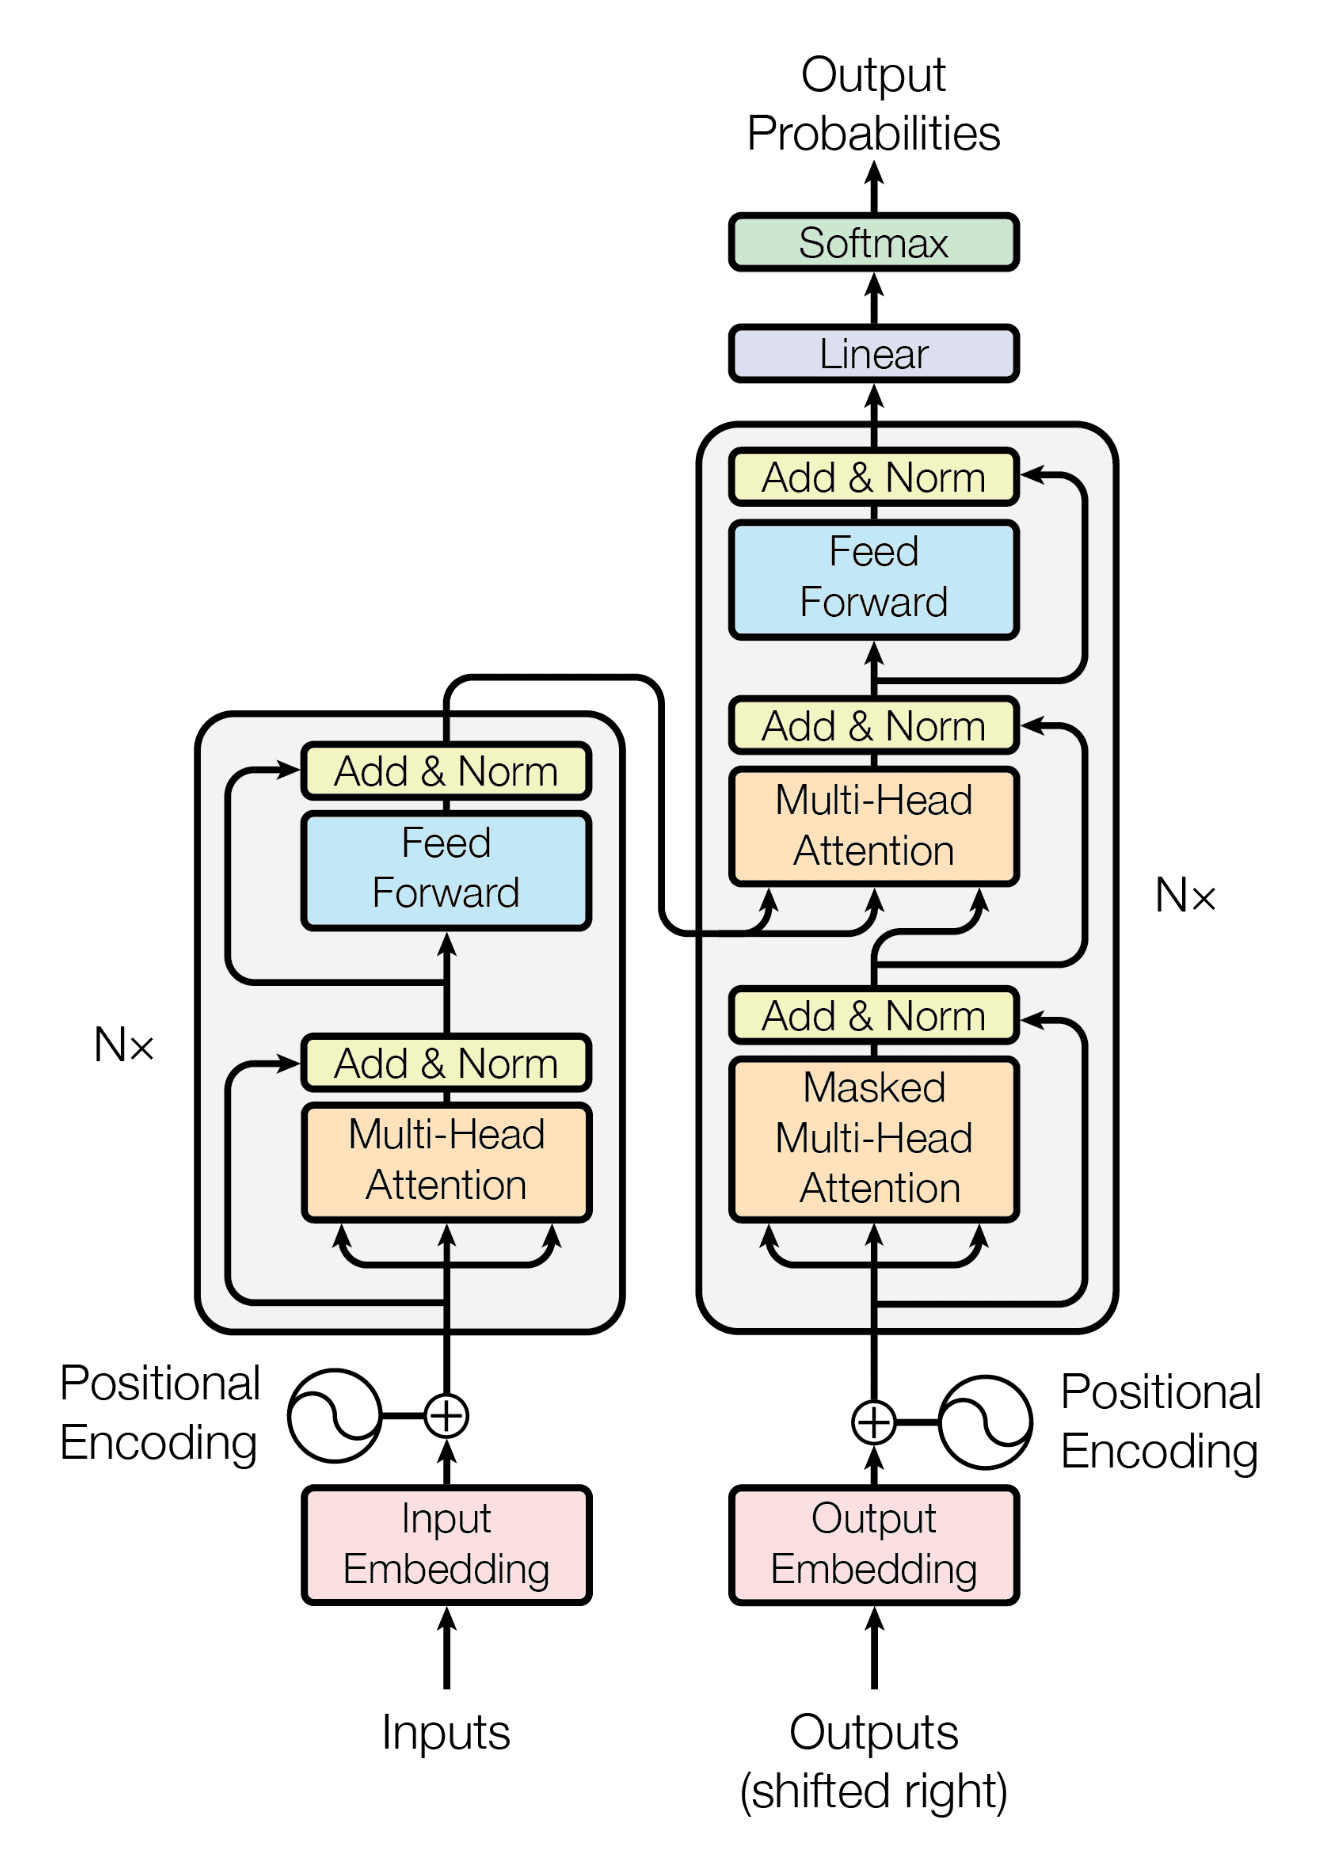
\includegraphics[width=0.55\textwidth]{figure/TransformerArch.png}
    \caption{La struttura Encoder-Decoder dell'architettura di un Transformer}
    \label{fig:tranArch}
\end{figure}

\section{Problemi con RNN e CNN}
Nei capitoli precedenti analizzando le reti convoluzionali e le reti ricorrenti, abbiamo notato come riscontrassero delle criticità:
\begin{itemize}
    \item \textbf{RNN}: processando i dati sequenzialmente, la difficoltà maggiore era parallelizzare i processi, un altro problema era quello relativo alla scomparsa/esplosione del gradiente su delle sequenze eccessivamente lunghe;
    \item \textbf{CNN}: queste reti neurali sono ottime per modelli locali, come per le immagini,  diventavano tuttavia molto inefficienti nel momento in cui si vuole catturare dipendenze molto lunghe, con la necessità pertanto di aumentarne la profondità.
\end{itemize}

Una delle soluzioni proposte è stata quella di usare il meccanismo dell'attenzione per modellare direttamente tutte le dipendenze in una singola sequenza, a prescindere dalla distanza, questa implementazione la ritroviamo nei Transformer.

\section{Visione ad alto livello}
Ci soffermeremo principalmente su un'applicazione dei Transformer, quella relativa alla traduzione automatica, un Transformer infatti, è in grado di prendere una frase in una lingua e generarne la traduzione in un'altra. A livello architetturale invece i Transformer si suddividono in due componenti principali:
\begin{itemize}
    \item \textbf{Encoder}: una pila di \textbf{N encoder} identici, nel paper in cui vengono presentati i Transformer ce ne sono 6, ognuno composto da due sottolivelli principali;
    \item \textbf{Decoder}: una pila di \textbf{N decoder} identici, anche in questo caso nel paper ce ne sono 6 specificando come il loro numero è strettamente collegato a quello degli encoder, anche i decoder, come gli encoder vengono strutturati in più sottolivelli.
\end{itemize}

Queste due componenti non condividono i pesi fra loro, analiziamo ora però i sottostrati degli Encoder, che sono fra loro indipendenti:

\begin{enumerate}
    \item \textbf{Self-Attention Layer}: consente all'encoder di "guardare" gli altri token presenti nella frase presa in input mentre ne elabora uno specifico per la parola presa in analisi;
    \item \textbf{Feed-Forward Neural Network}: l'output del self attention layer, viene passato a questo layer il quale applica indipendentemente le sue modifiche a ciascuna posizione del token di una frase.
\end{enumerate}

Il decoder, include gli stessi due livelli presenti nell'encoder, e ne aggiunge uno ulteriore fra i due, chiamato \textbf{Encoder-Decoder Attention}, il quale si sofferma sulle parti più rilevanti della frase mandata in input.

\begin{figure}
    \centering
    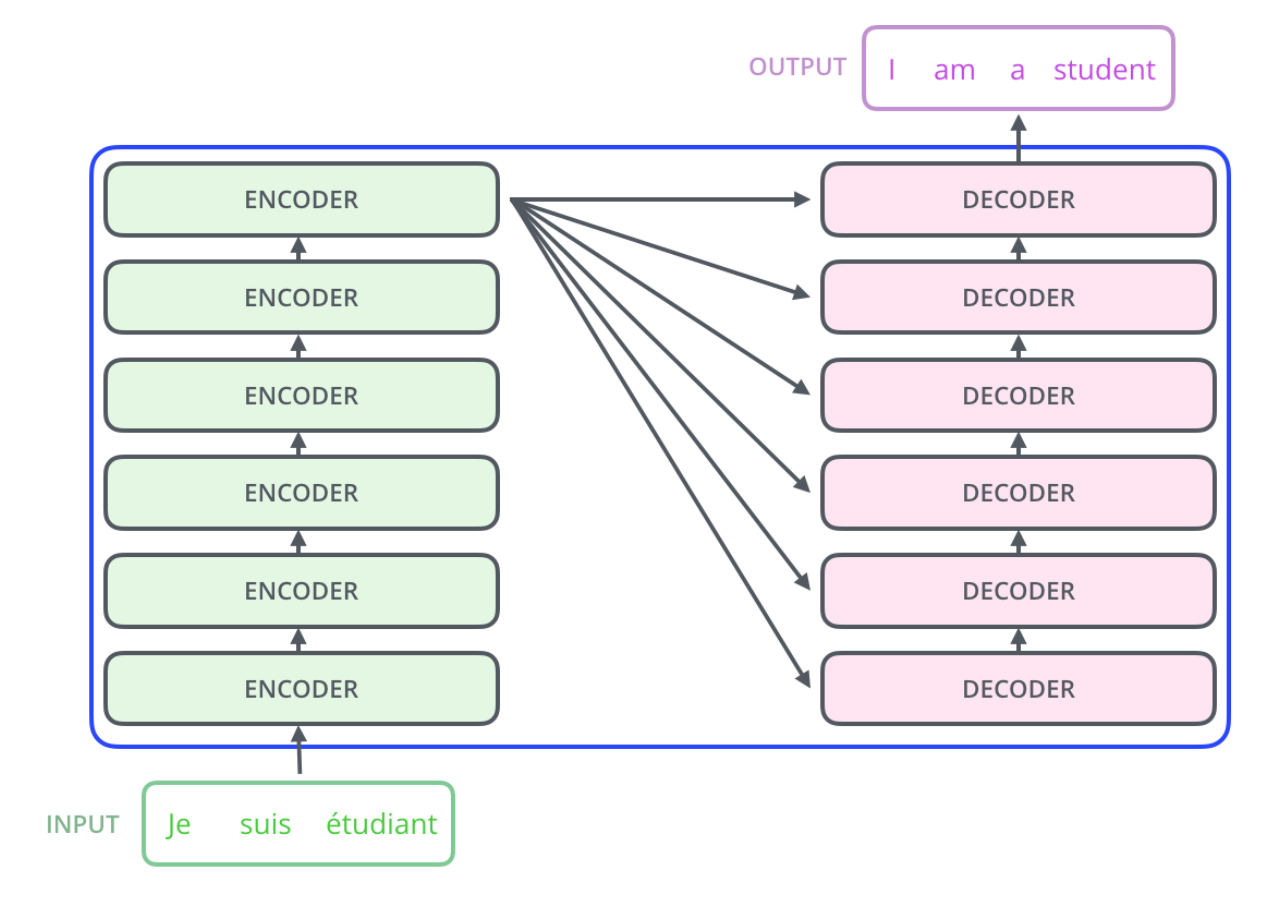
\includegraphics[width=\textwidth]{figure/EncDecTransformers}
    \caption{Rappresentazione ad alto livello di un'architettura di un Transformer, focalizzandosi principalmente sulla parte in cui vi sono gli Encoder e i Decoder}
    \label{fig:EncDecTrasf}
\end{figure}

\section{Introduzione ai Tensori}

Ogni parola data come input viene trasformata in un vettore di dimensione 512, tramite l'utilizzo di un algoritmo di embedding. L'embedding avviene solo nel primo encoder, mentre gli encoder successivi ricevono come input gli output del layer sottostante. La lunghezza della frase, dunque il numero di vettori è un \textit{iperparametro}, il quale può essere impostato durante la progettazione. Una volta effettuato l'embedding delle nostre parole, esse scorreranno all'interno dei vari layer presenti nei nostri encoder. Ogni parola segue un suo percorso indipendente all'interno dell'encoder, inoltre vengono create delle relazioni fra questi percorsi tramite il meccanismo dell'attenzione, mentre nel layer di feed-forward, non ci sono dipendenze e ciò permette l'esecuzione parallela, aumentando l'efficienza.

\section{Self-Attention}

Come già accennato in precedenza adesso, entriamo nel dettaglio per approfondire il così detto \textit{meccanismo dell'attenzione}, questo meccanismo è l'effettiva rivoluzione che viene proposta nel paper precedentemente citato, permettendo a ogni parola di ponderare la rilevanza della altre parole in una frase. Prendiamo in considerazione una frase in cui vi è un soggetto sottointesto, per noi umani risulta molto semplice determinarne chi è il soggetto, diversamente per una macchina questo risulta un meccanismo arduo. Se ci fosse un qualcosa, che permette di mettere in relazione i vari token presenti in una frase, e riuscire a determinarne le relazioni capendo effettivamente il soggetto della frase aiuterebbe molto. Infatti il \textit{self-attention mechanism}, fa proprio ciò, mettendo in relazione i singoli token e arginando questa difficoltà.

\begin{figure}
    \centering
    \includegraphics[width=0.65\textwidth]{figure/selfAttention}
    \caption{Nell'immagine possiamo vedere le singole relazioni, rappresentate dalle linee di connessione della parola \textit{it} con le altre parole della frase, più spessa è la linea, più solida riuslta essere la relazione.}
    \label{fig:selfAtt}
\end{figure}


\subsection{Self-Attention in dettaglio}

La prima fase per il calcolo della self-attention consiste nel creare ben tre vettori a partire da ogni vettore mandato in input agli encoder, nel nostro caso non sarebbero altro che gli embedding delle singole parole. Dunque vengono generati un vettore detto Query (Q), un vettore detto Key (K) e infine un vettore detto Value (V). La Self-Attention, si basa su una semplice idea: 
\begin{quote}
    Ogni parola (Query) cerca "parole chiavi" (Key), tra tutte le parole per capire da chi e quanta informazione prendere (Value).
\end{quote}

Ogni token ha un Embedding, tutti questi vengono racchiusi in un vettore degli Embedding $E$, il quale viene moltiplicato per tre matici differenti: $W^Q$, $W^K$, $W^V$, tre matrici apprese durante il training, inizialmente inizializzate a valori piccoli le quali ci permettono di ottenere rispettivamente il Query vecotr, il Key vector e il Value vector.

\begin{equation}
    Q = E \times W^Q\,,\qquad K=E\times W^K\,,\qquad V=E\times W^V
\end{equation}

Una volta calcolati i tre vettori, non facciamo altro che effettuare dei confronti, in primis calcoliamo l'affinità fra ogni $Q$ con tutte le $K$, successivamente dividiamo per la radice quadrata del valore della dimensione di $Q$ e $K$, applichiamo la funzione $\operatorname{softmax}$ che ci dirà quanto sono compatibili, e infine moltiplichiamo tutto ciò con i valori $V$, in modo tale che il token corrente mixa informazioni dagli altri token in base all'attenzione.

\begin{equation}
    \operatorname{Attention}(Q,K,V) = \operatorname{softmax}\left(\frac{Q\,K^T}{\sqrt{d_k}}\right)\,V 
\end{equation}


\subsubsection{Esempio di calcolo}
Adesso prendiamo in analisi un esempio di calcolo prendendo in considerazione di partire dalla seguente frase:
\begin{quote}
    Il gatto dorme.
\end{quote}

Ogni parola avrà un embedding corrispondente, immaginiamo in questo caso dei numeri molto semplici per facilità di comprensione:

\begin{table}[h!]
    \centering
    \caption{Embedding vettoriali delle parole}
    \begin{tabular}{@{}lc@{}}
        \toprule
        \textbf{Parola} & \textbf{Embedding} \\
        \midrule
        Il     & $\left[1, 0\right]$ \\
        Gatto  & $\left[0, 1\right]$ \\
        Dorme  & $\left[1, 1\right]$ \\
        \bottomrule
    \end{tabular}
\end{table}

Supponiamo che le nostre matrici siano delle matrici semplici, delle matrici identità o piccole trasformazioni, in modo tale che il prodotto fra matrici non sia eccessivamente complicato, nel nostro caso consideriamo che siano tutte matrici identità. Pertanto ottenendo i valori per ogni singola parola $Q,K,V$ saranno tutti la copia della singola parola presa in considerazione. Passo al confronto fra le singole parole, effettuando il prodotto scalare fra il vettore $Q$ e il vettore $K$ :

\begin{table}[h!]
    \centering
    \caption{Prodotti scalari tra Query e Key per ogni coppia di parole}
    \begin{tabular}{@{}lccc@{}}
        \toprule
        \textbf{Da} & \textbf{Il ($[1, 0]$)} & \textbf{Gatto ($[0, 1]$)} & \textbf{Dorme ($[1, 1]$)} \\
        \midrule
        Il ($Q = [1, 0]$)     & 1 & 0 & 1 \\
        Gatto ($Q = [0, 1]$)  & 0 & 1 & 1 \\
        Dorme ($Q = [1, 1]$)  & 1 & 1 & 2 \\
        \bottomrule
    \end{tabular}
\end{table}


Effettuati questi prodotti scalari, dividerò i singoli valori per la radice quadrata della grandezza dei vettori, nel nostro caso per $\sqrt{2}$ e li immetto all'interno di una \textbf{softmax}, la quale ci darà dei pesi che sommati ci porteranno a un valore unitario. Essa enfatizzerà l'importanza delle parole più rilevanti, rendendo il modello capace di contestualizzare correttamente ogni termine.

\subsubsection{L'analogia delle cartelle}
Supponiamo di avere un armadietto, al quale interno ci sono numerose cartelle, il nostro obbiettivo è trovare la cartella corrispondente al post-it che abbiamo in mano (Figura~\ref{fig:folderAn}). Il post-it in questo caso non è altro che la nostra query, le key non sono altro che l'identificativo della nostra cartella, dunque il loro nome. Una volta che trovo una corrispondenza fra la cartella e il nostro post-it, prendiamo la cartella e la poniamo al di fuori del nostro armadietto e aprendola al suo interno ci troviamo qualcosa, la quale rappresenta il value. Moltiplicare il vettore query per ogni vettore chiave produce un punteggio per ogni cartella, il quale punteggio maggiore mette in evidenza la corrispondenza più quotata fra le due parole.

\begin{figure}
    \centering
    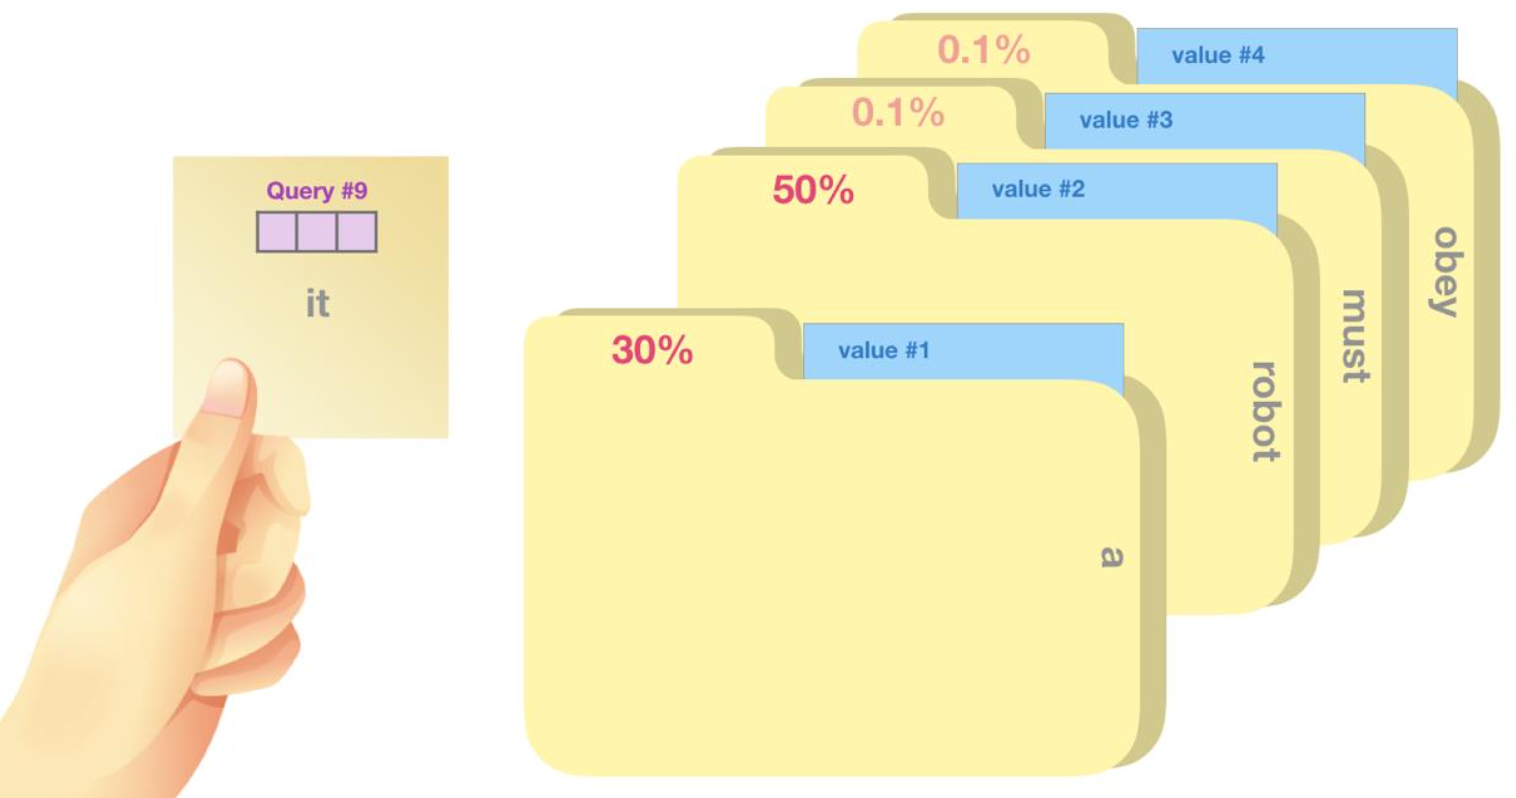
\includegraphics[width=0.75\textwidth]{figure/FoldeAnalogy.png}
    \caption{Rappresentazione dell'analogia delle cartelle, nel quale si rappresentano i tre vettori, query vector come il post-it, key vector come l'identificativo di ogni cartella, value vector come il valore all'interno di ogni cartella, ogni cartella ha un punteggio che mappa la percentuale di corrispondenza.}
    \label{fig:folderAn}
\end{figure}

\section{Multi-Head Attention}

Il meccanismo di self-attention può essere ulteriormente potenziato tramite l'introduzione della \textbf{Multi-Head Attention}, una tecnica che migliora l'efficacia dell'attenzione secondo due principali direttrici:

\begin{enumerate}
\item Amplia la capacità del modello di focalizzarsi su posizioni differenti nella sequenza di input. Ad esempio, il vettore $z_1$ associato alla prima parola potrebbe rappresentare un misto di tutte le codifiche, ma al contempo essere fortemente influenzato dalla parola stessa;
\item Introduce molteplici \emph{sottospazi di rappresentazione} all'interno dello stesso livello di attenzione. Invece di utilizzare un singolo insieme di matrici di peso per $Q$, $K$ e $V$, si impiegano più insiemi distinti, ciascuno inizializzato in modo indipendente. Al termine dell’addestramento, ogni insieme proietta gli embedding d’ingresso in uno spazio latente diverso, catturando così vari aspetti delle relazioni tra parole.
\end{enumerate}

Questo meccanismo introduce diverse \emph{teste di attenzione} (\emph{heads}), ognuna delle quali applica il calcolo di attenzione in modo indipendente, utilizzando parametri distinti. Ogni testa analizza l’input da una prospettiva differente, permettendo al modello di cogliere vari tipi di relazioni semantiche e sintattiche tra le parole. Alla fine, i vettori prodotti da ciascuna testa ($z_i$) vengono concatenati e successivamente proiettati in uno spazio comune tramite una matrice di pesi addizionale, $W_o$, appresa durante l’addestramento. Questo passaggio ha lo scopo di restituire un singolo vettore di output da fornire al livello feed-forward della rete.

\subsubsection{Esempio}

Consideriamo nuovamente una frase semplice per illustrare il funzionamento:

\begin{quote}
Il gatto che inseguiva il topo miagolava.
\end{quote}

Focalizziamoci sulla parola \textit{miagolava}. Essa intrattiene relazioni diverse con le parole precedenti: \textit{gatto} è il soggetto che compie l’azione, \textit{inseguiva} rappresenta un’azione precedente, mentre \textit{topo} non ha relazione semantica diretta con l’azione del miagolare. Una singola testa di attenzione faticherebbe a modellare contemporaneamente tutte queste relazioni. La Multi-Head Attention risolve questo problema distribuendo l’analisi su più teste: ciascuna può concentrarsi su un tipo specifico di relazione. Alcune teste potrebbero enfatizzare il legame semantico tra soggetto e verbo, altre potrebbero evidenziare correlazioni sintattiche o ignorare completamente parole irrilevanti. Dal punto di vista grafico, ciò rende la rappresentazione visiva del meccanismo più complessa rispetto al caso della self-attention classica (Figura~\ref{fig:selfAtt}), ma allo stesso tempo più espressiva e potente (Figura~\ref{fig:multiHeadAtt}).

\begin{figure}
    \centering
    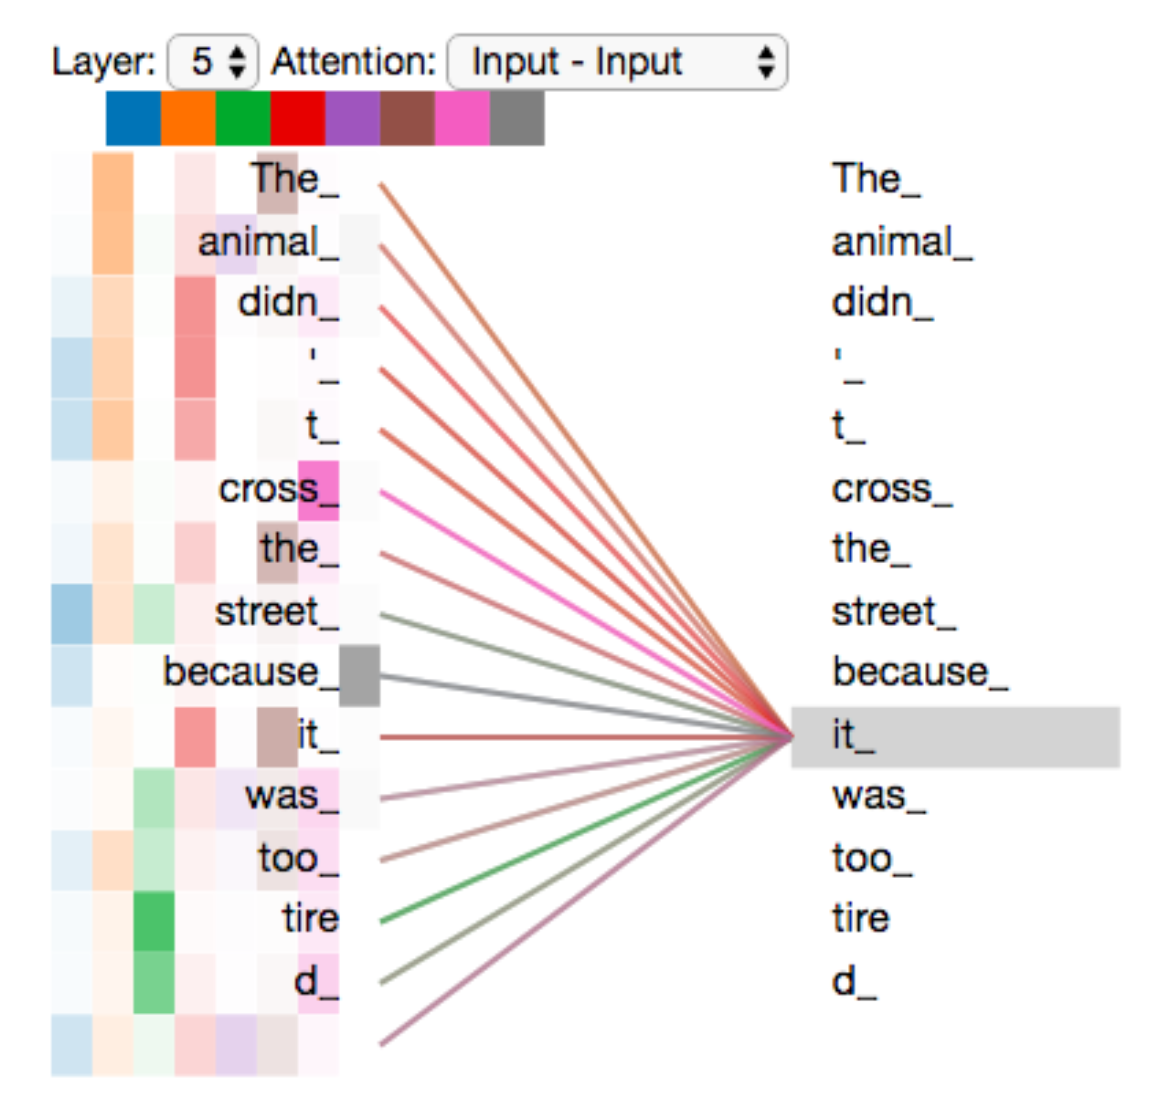
\includegraphics[width=0.5\textwidth]{figure/MultiHeadAttention}
    \caption{Esempio visivo della Multi-Head Attention: ogni testa stabilisce relazioni differenti tra la parola "it" e le altre nel contesto, evidenziate con colori distinti.}
    \label{fig:multiHeadAtt}
\end{figure}

\section{Positional Encoding}

Una limitazione intrinseca del meccanismo di self-attention è la mancanza di una nozione esplicita di ordine all'interno della sequenza. A differenza delle reti ricorrenti, i Transformer processano gli input in parallelo, senza tenere conto, di per sé, della posizione delle parole nella frase. Per colmare questa lacuna, il modello introduce un meccanismo chiamato \textbf{Positional Encoding}. Esso consiste nell’aggiunta, ad ogni embedding di input, di un vettore che codifica la posizione della parola nella sequenza. In questo modo, si conferisce al modello un senso dell’ordine, fondamentale per comprendere la struttura linguistica. I vettori di positional encoding non sono appresi durante l'addestramento, bensì definiti in modo deterministico secondo un pattern sinusoidale. La loro struttura è tale da garantire che, dopo la proiezione nei vettori $Q$, $K$ e $V$, le posizioni relative tra parole risultino distinguibili anche nel prodotto scalare dell'attenzione. In particolare, i vettori vengono definiti dalle seguenti funzioni:

\begin{equation}
    PE_{(\operatorname{pos},,2i)} = \sin\left(\frac{\operatorname{pos}}{10000^{\frac{2i}{d_{\operatorname{model}}}}}\right), \quad
    PE_{(\operatorname{pos},,2i+1)} = \cos\left(\frac{\operatorname{pos}}{10000^{\frac{2i}{d_{\operatorname{model}}}}}\right)
\end{equation}

Qui $\operatorname{pos}$ rappresenta la posizione della parola nella sequenza, $i$ è l'indice della dimensione dell'embedding, e $d_{\operatorname{model}}$ indica la dimensione totale del vettore. Ogni dimensione dell’embedding segue quindi un’onda sinusoidale con frequenza diversa, che cresce in progressione geometrica da $2\pi$ fino a $1000 \cdot 2\pi$. Questa scelta progettuale è motivata dall’intuizione che le posizioni relative tra parole possano essere modellate in modo lineare. Infatti, dato un offset $k$, il positional encoding associato alla posizione $\operatorname{pos} + k$ può essere espresso come una funzione lineare del positional encoding di $\operatorname{pos}$, facilitando il compito del modello nel cogliere le distanze relative tra parole.
\begin{figure}[hbtp]
    \centering
    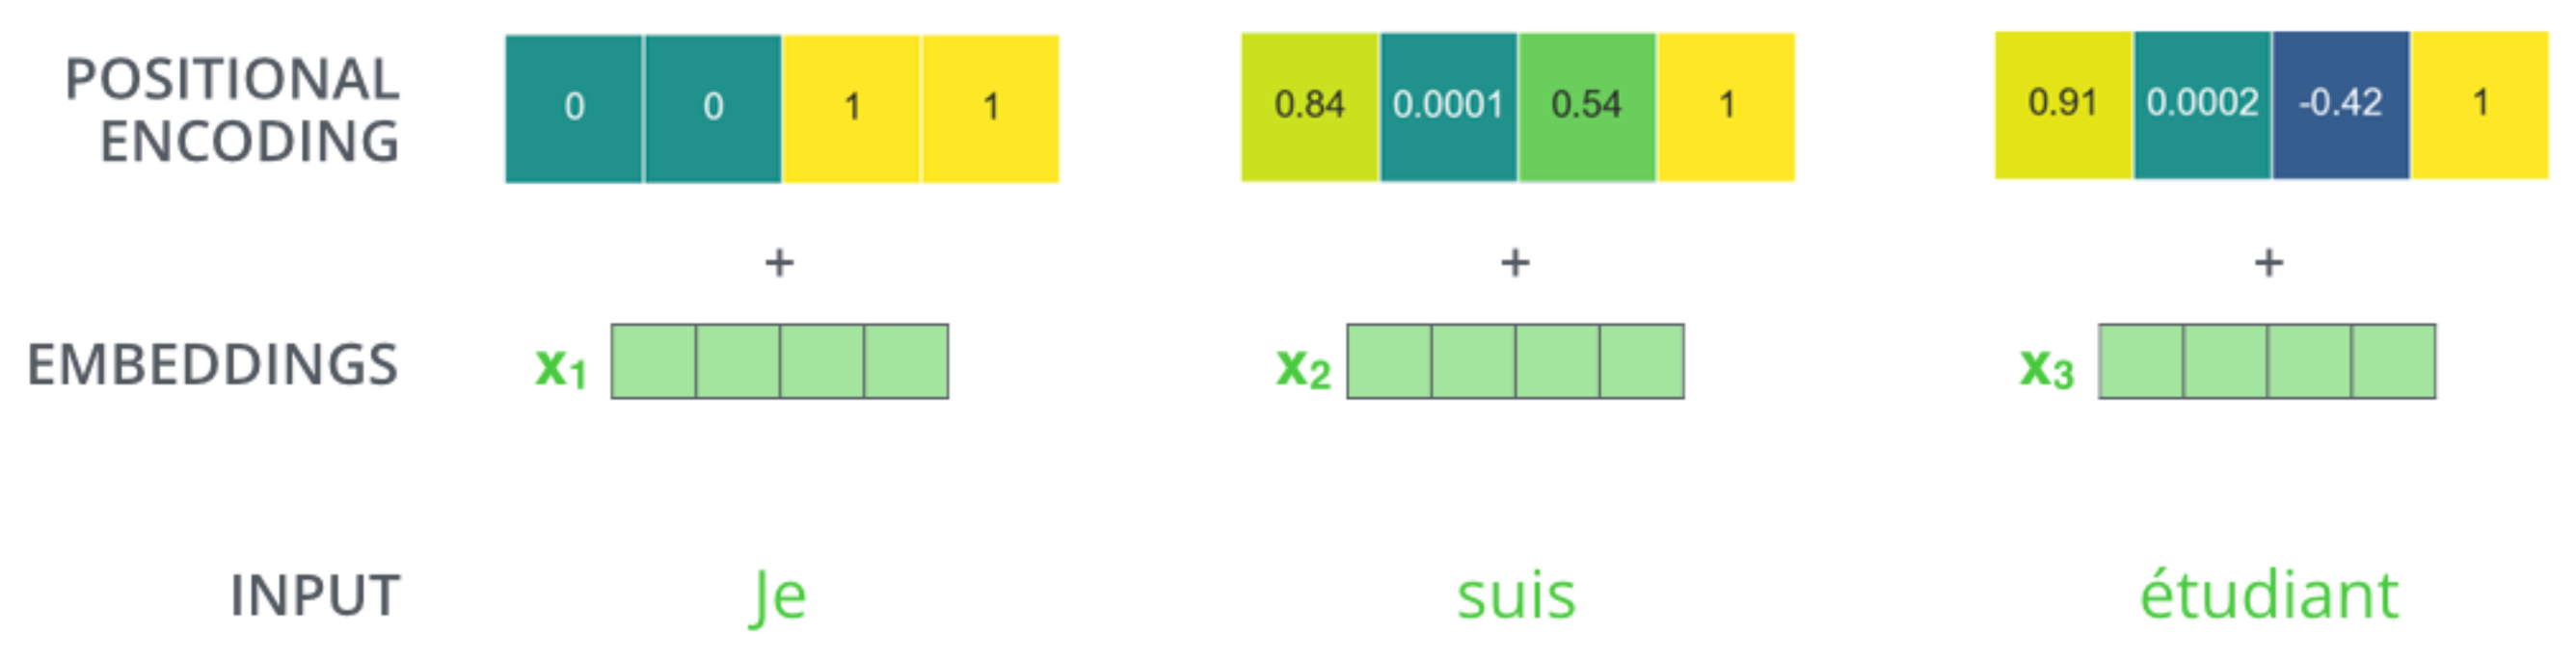
\includegraphics[width=0.85\textwidth]{figure/PositionalEncoding}
    \caption{Esempio di Positional Encoding per embedding a 4 dimensioni. Ogni curva corrisponde a una dimensione del vettore.}
    \label{fig:posEncoding}
\end{figure}
Esperimenti condotti nel lavoro originale hanno dimostrato che queste funzioni sinusoidali risultano efficaci almeno quanto i positional encoding appresi, ma presentano il vantaggio di non introdurre ulteriori parametri nel modello.

\section{Residual Connections}

Nel contesto dell’architettura Transformer, le \textbf{connessioni residue} (o \textit{residual connections}) svolgono un ruolo cruciale nell’agevolare l’addestramento di reti neurali profonde e nel garantire una maggiore stabilità numerica durante la propagazione del segnale. Una connessione residua è un meccanismo architetturale che permette di sommare direttamente l’input $x$ di uno strato con il suo output trasformato $F(x)$. Formalmente, l’output risultante è dato da:

\begin{equation}
    \operatorname{Output} = F(x) + x
\end{equation}

Tale strategia è stata introdotta originariamente nelle reti ResNet, e successivamente adottata nei Transformer per i benefici che comporta in termini di stabilità e capacità di apprendimento. Essa consente al flusso informativo di "saltare" uno o più livelli, riducendo così il rischio che le trasformazioni applicate lungo la rete degradino l’informazione iniziale. Nel Transformer, ciascun blocco (sia dell’encoder che del decoder) include due moduli principali: il meccanismo di \textit{Multi-Head Attention} e il sottoblocco \textit{Feed-Forward}. Entrambi questi moduli sono avvolti da una struttura chiamata \textbf{Add \& Norm}, composta da una connessione residua e da una successiva normalizzazione (tipicamente, \textit{Layer Normalization}). In questa struttura, l’input originale viene sommato all’output del modulo, e il risultato viene poi normalizzato. Questo schema è illustrato in Figura~\ref{fig:ResAddon}.
\begin{figure}
    \centering
    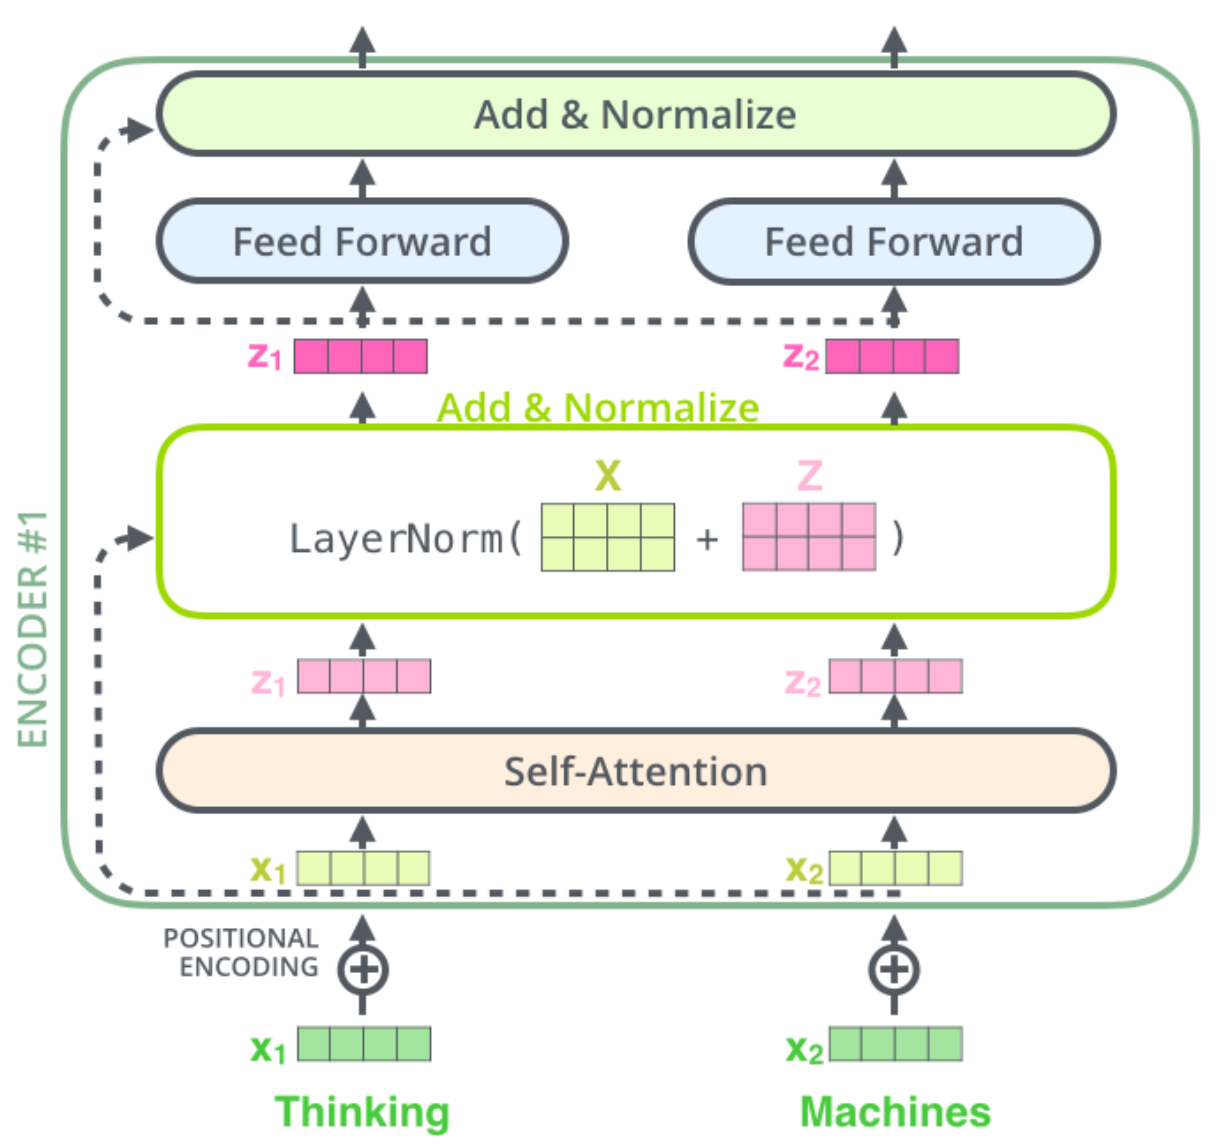
\includegraphics[width=0.6\textwidth]{figure/ResidualAddon.png}
    \caption{Struttura del blocco Add \& Norm, che incapsula un modulo con connessione residua e normalizzazione.}
    \label{fig:ResAddon}
\end{figure}
L’integrazione delle connessioni residue all’interno del modello comporta numerosi vantaggi:
\begin{itemize}
    \item \textbf{Mitigazione del problema del gradiente che scompare}: facilitano la retropropagazione del gradiente anche in reti molto profonde, migliorando la stabilità dell’addestramento;
    \item \textbf{Preservazione dell’informazione originale}: permettono di conservare componenti essenziali dell’input che potrebbero essere alterate dalle trasformazioni non lineari successive;
    \item \textbf{Facilitazione dell’apprendimento}: rendono più agevole l’apprendimento di funzioni identitarie o prossime all’identità, accelerando la convergenza durante l’ottimizzazione.
\end{itemize}
Possiamo interpretare le connessioni residue come delle vere e proprie "corsie preferenziali" per il flusso informativo: il modello può scegliere se utilizzare l’informazione trasformata, conservarla intatta, o combinare entrambe. Questo è particolarmente utile in presenza di molteplici strati successivi, dove l’accumulo di trasformazioni può facilmente portare a una perdita di contenuto semantico rilevante.

\section{Decoder}

Il \textbf{decoder} ha il compito di generare la sequenza di output a partire dalla rappresentazione codificata dell’input fornita dall’encoder. In particolare, l’output dell’ultimo strato dello stack degli encoder viene trasformato in un insieme di vettori chiave ($K$) e valore ($V$), che saranno utilizzati in ogni strato del decoder all’interno del modulo \textit{Encoder-Decoder Attention}. Questo meccanismo permette al decoder di concentrarsi selettivamente su specifiche porzioni della sequenza di input, fornendo così una forma di allineamento tra input e output. Il processo si ripete iterativamente finché non viene generato un simbolo speciale di fine sequenza (\texttt{<eos>}), che segnala al modello il termine della generazione. Ad ogni passo, l’output prodotto dal decoder viene reinserito come input per il passo successivo, e tale operazione prosegue lungo la pila di decoder in maniera analoga a quanto accade per l’encoder. Anche nel decoder, viene incorporata l’informazione posizionale, attraverso apposite rappresentazioni, per permettere al modello di distinguere l’ordine delle parole nella sequenza.
\begin{figure}
    \centering
    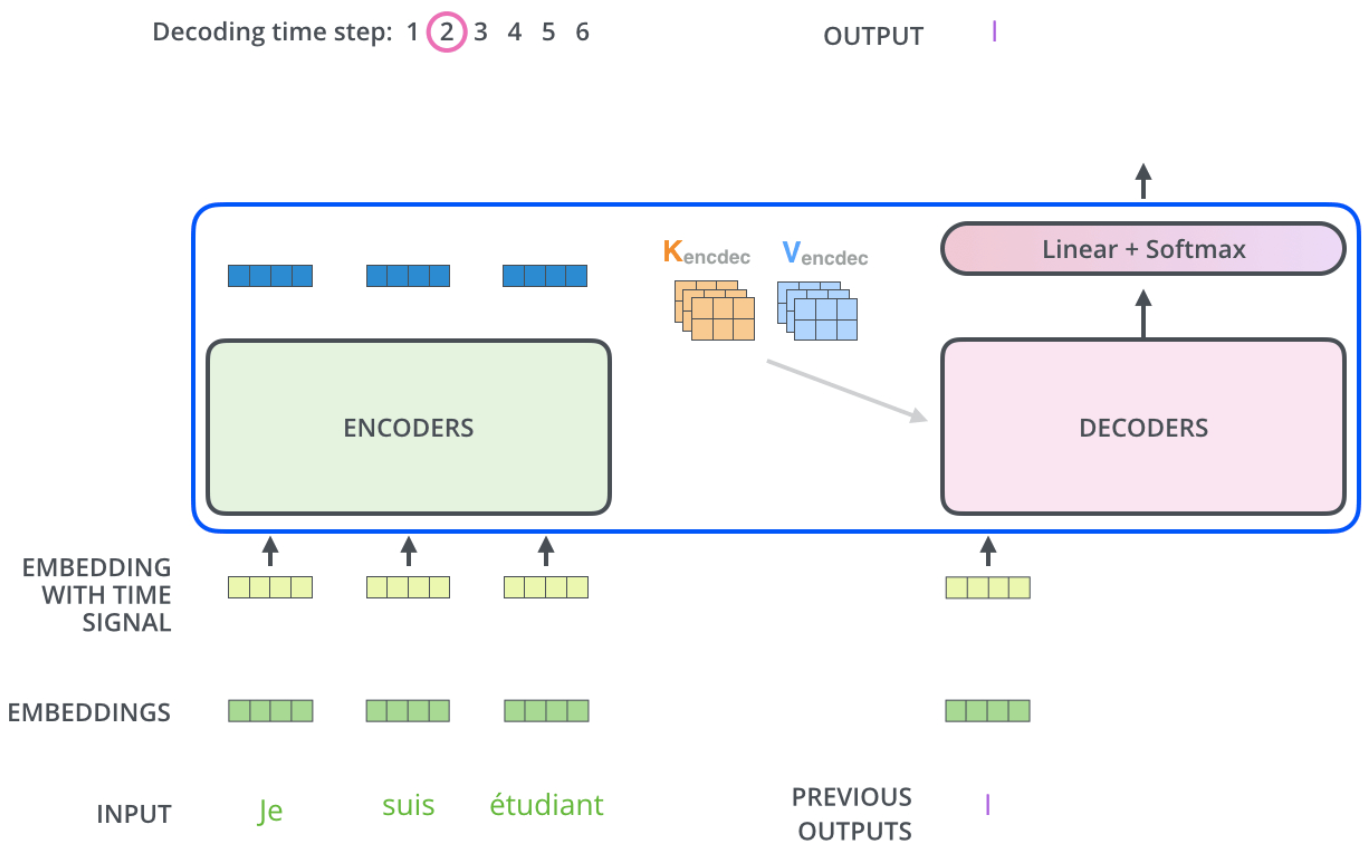
\includegraphics[width=\textwidth]{figure/DecoderSample.png}
    \caption{Esempio del processo di generazione nel decoder al secondo step temporale. Nel primo step è stata generata la parola \textit{I} come traduzione di \textit{je}.}
    \label{fig:DecSam}
\end{figure}
Una differenza sostanziale rispetto al funzionamento dell’encoder risiede nel meccanismo di \textbf{self-attention} impiegato nel decoder. In questo caso, l’attenzione è \textit{mascherata} per evitare che il modello acceda a posizioni future della sequenza di output. Più precisamente, le posizioni successive a quella corrente vengono oscurate (mascherate) assegnando loro un valore $-\infty$ prima dell'applicazione della funzione $\operatorname{softmax}$, così da annullarne il contributo. Il modulo \textit{Encoder-Decoder Attention}, invece, opera in maniera analoga alla self-attention multi-testa, con la differenza che le matrici $K$ e $V$ provengono direttamente dall’output dello stack degli encoder, mentre le matrici $Q$ (Query) vengono calcolate a partire dallo strato sottostante del decoder stesso.

\subsection{Final Layer e Softmax}

Lo stack dei decoder, al termine della generazione, produce un vettore continuo (un vettore di float), che deve essere convertito in una parola del vocabolario. A questo scopo intervengono due componenti finali: il \textbf{Final Linear Layer} e il \textbf{Softmax Layer}. Il \textit{Final Linear Layer} è una rete completamente connessa che trasforma il vettore di rappresentazione generato dal decoder in un \textbf{vettore di logit}, detto anche \textit{logits vector}. Questo vettore ha una dimensione pari alla cardinalità del vocabolario: ad esempio, se il modello gestisce un vocabolario di 10.000 parole, il vettore sarà lungo 10.000, e ciascun valore rappresenterà il punteggio non normalizzato associato a una specifica parola. Il \textit{Softmax Layer} converte questo vettore di logit in una distribuzione di probabilità: tutti i valori risultanti saranno positivi e la loro somma sarà pari a uno. L’indice con la probabilità più alta indicherà la parola da generare in quello specifico time step.

\begin{figure}
    \centering
    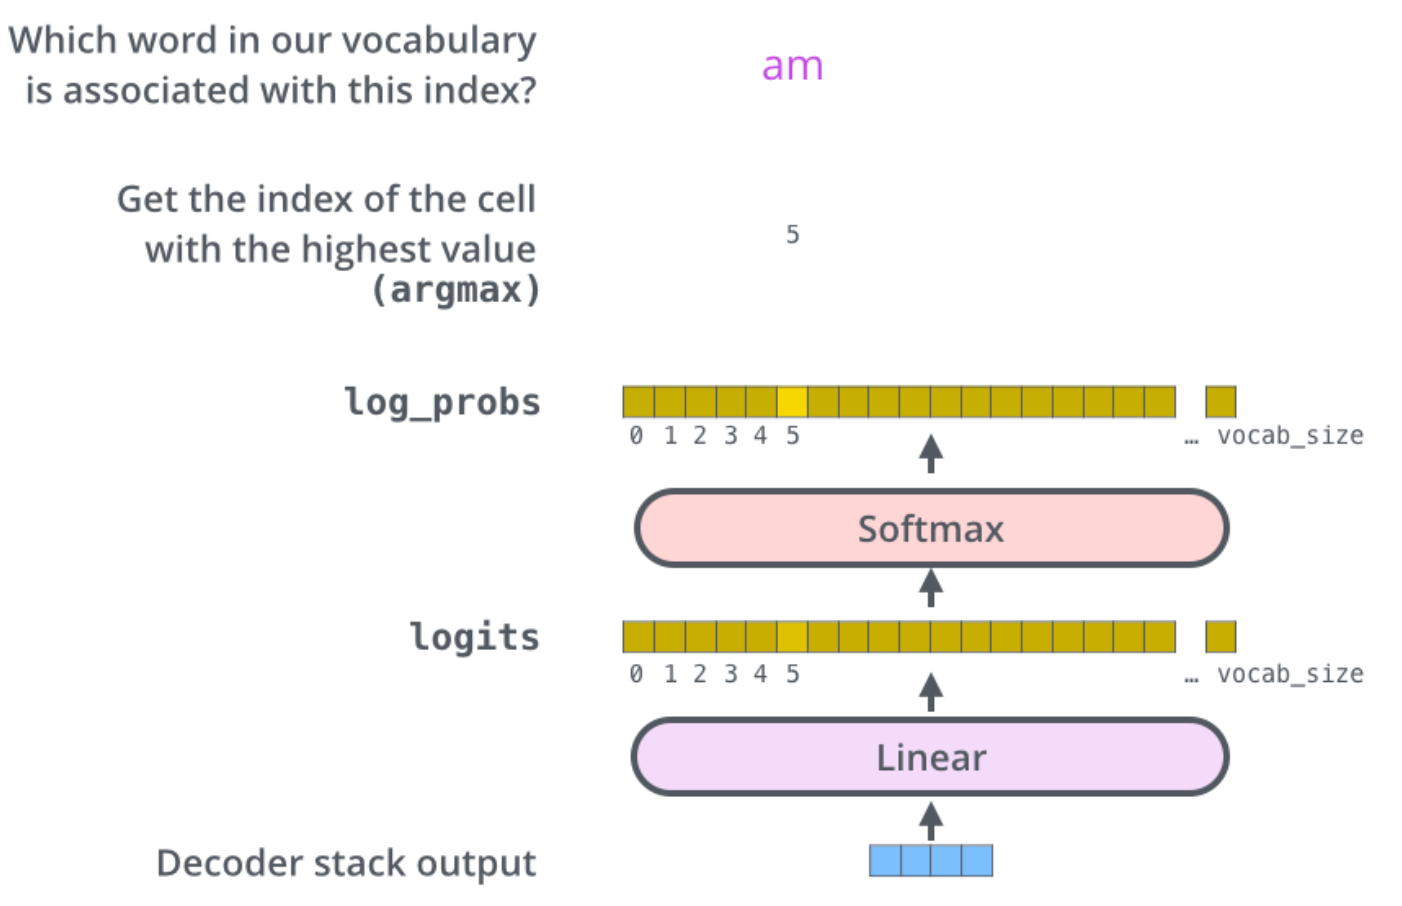
\includegraphics[width=0.75\textwidth]{figure/FinalLayer.png}
    \caption{Struttura dei layer finali del decoder nel Transformer, che trasformano la rappresentazione vettoriale in una parola.}
    \label{fig:FinLay}
\end{figure}

\section{Allenamento di un Transformer}

Durante la fase di \textbf{addestramento}, il Transformer esegue un \textit{forward pass} sui dati forniti. Poiché il dataset di training è etichettato, è possibile confrontare le uscite del modello con i target attesi, valutando così la qualità delle predizioni. In presenza di discrepanze tra output previsto e desiderato, si procede con un aggiornamento dei pesi tramite backpropagation, al fine di minimizzare l’errore e migliorare la capacità predittiva del modello. I vocabolari utilizzati nei Transformer contengono generalmente un numero elevato di parole, oltre a simboli speciali come \texttt{<eos>} (\textit{end of sequence}), che indica al modello il termine della sequenza da generare. Prima dell’allenamento, ogni parola viene mappata su un vettore numerico tramite un processo di \textit{preprocessing}. Una rappresentazione comune è la \textbf{One-Hot Encoding}, in cui ogni parola è rappresentata da un vettore con tutti zeri, tranne un valore pari a uno in corrispondenza della posizione associata alla parola nel vocabolario. Nelle prime fasi di training, un modello non ancora addestrato produce uscite casuali e scorrelate dal target. L’obiettivo dell’addestramento è dunque quello di guidare il modello a produrre, per ciascun time step, una distribuzione di probabilità in cui la parola attesa abbia la probabilità più alta. Ogni distribuzione è un vettore di lunghezza pari al numero di parole nel vocabolario, e la sequenza di distribuzioni dovrebbe idealmente riflettere la sequenza di parole target. In particolare, ci si aspetta che la prima distribuzione assegni il valore di probabilità più alto alla prima parola desiderata, la seconda alla seconda parola, e così via, fino all’ultima distribuzione, in cui la probabilità più alta dovrebbe corrispondere al token \texttt{<eos>}, segnalando la fine della sequenza.

\begin{figure}
    \centering
    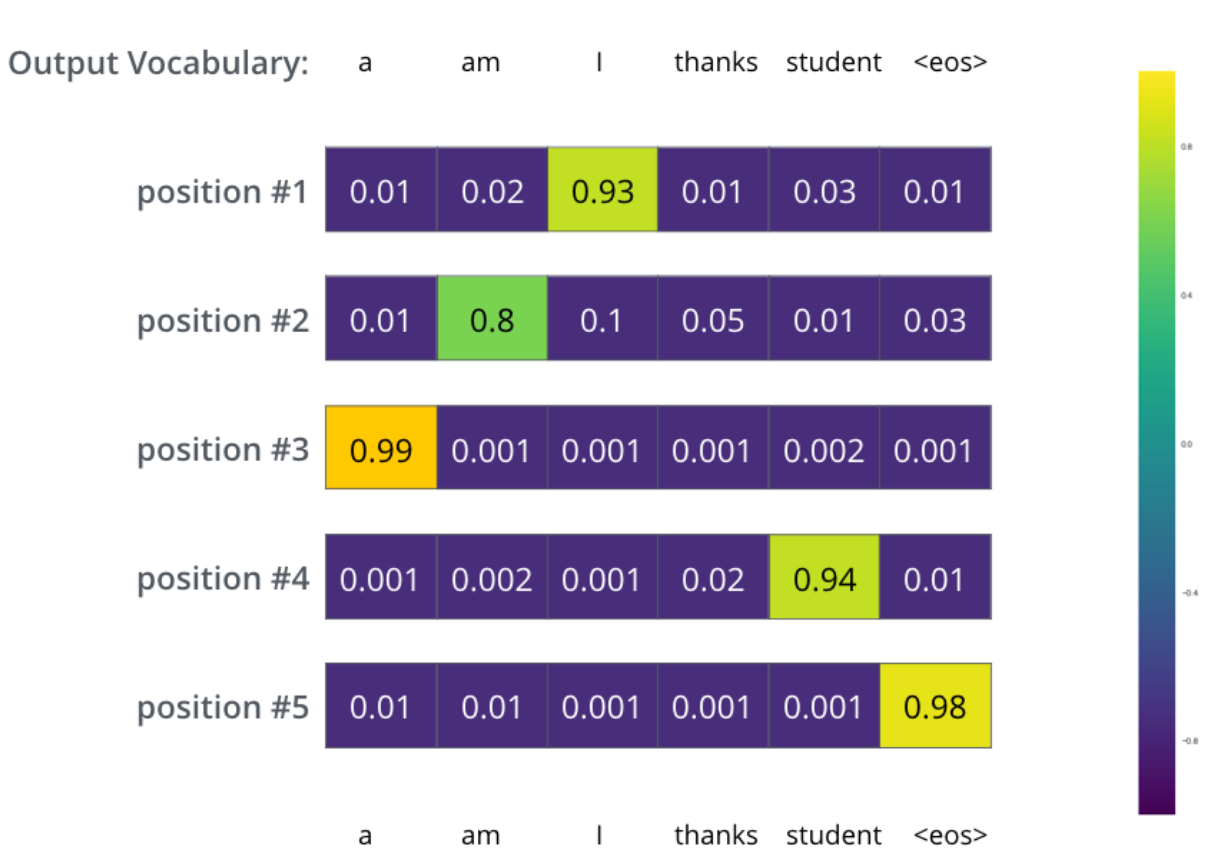
\includegraphics[width=0.8\textwidth]{figure/TrainExpectation}
    \caption{Distribuzioni di probabilità prodotte dal decoder: ogni posizione temporale è associata a una distribuzione su tutto il vocabolario, e ci si aspetta che la parola target sia quella con la probabilità massima.}
    \label{fig:trainExp}
\end{figure}

\section{Oltre la struttura base del Transformer}

Con la comprensione completa dell'architettura originaria del Transformer, siamo ora pronti ad analizzare alcune delle estensioni fondamentali che hanno reso questo modello uno standard de facto nel campo del deep learning. In particolare, approfondiremo come il Transformer venga adattato a contesti specifici mediante il \textbf{fine-tuning}, quali siano le sue principali \textbf{applicazioni} in scenari reali e accademici, e infine esamineremo alcune delle \textbf{varianti architetturali} che ne estendono le potenzialità, spesso superandone i limiti originali.

\section{Fine-Tuning del Transformer}

Il \textbf{fine-tuning} è una tecnica di apprendimento trasferito (\textit{transfer learning}) ampiamente adottata nel contesto dei Transformer, che consente di adattare un modello pre-addestrato a un compito specifico. Il modello viene inizialmente addestrato su un vasto corpus general-purpose (come Wikipedia o Common Crawl), apprendendo rappresentazioni linguistiche ricche e versatili. Successivamente, viene ottimizzato su un dataset mirato, spesso molto più piccolo, relativo a un task specifico (ad esempio, classificazione di sentiment, riconoscimento di entità, generazione di codice, ecc.).

Il processo si articola come segue:
    \begin{enumerate}
        \item \textbf{Pretraining}: il modello viene addestrato in maniera auto-supervisionata su un task generale (e.g. \textit{masked language modeling} o \textit{causal language modeling}).
        \item \textbf{Fine-tuning supervisionato}: si sostituisce o si estende la testa del modello con uno o più layer adatti al task target (es. classificazione), e si effettua un training supervisionato con gradient descent.
    \end{enumerate}

Uno degli aspetti cruciali del fine-tuning è la scelta del \textit{learning rate}: un tasso troppo elevato potrebbe sovrascrivere le rappresentazioni apprese nel pretraining; al contrario, uno troppo basso potrebbe non fornire l'adattamento desiderato.

\section{Applicazioni del Transformer}

L'architettura Transformer è stata adottata in una vasta gamma di applicazioni, sia in ambito linguistico che in domini non testuali. Tra le principali:

\begin{itemize}
    \item \textbf{Natural Language Processing (NLP)}: è il dominio originario del Transformer, dove viene impiegato in:
    \begin{itemize}
        \item Traduzione automatica (e.g. Google Translate)
        \item Generazione di testo (e.g. ChatGPT, GPT-4)
        \item Analisi del sentiment
        \item Estrazione di entità (NER)
        \item Riassunto automatico
    \end{itemize}
    \item \textbf{Visione artificiale (CV)}: con modelli come Vision Transformer (ViT), l'architettura viene adattata al dominio visivo per compiti come classificazione, segmentazione e object detection.\item \textbf{Bioinformatica e Chimica Computazionale}: i Transformer vengono utilizzati per la modellazione di sequenze proteiche, il drug discovery, e la predizione di interazioni molecolari.
    \item \textbf{Codice e programmazione automatica}: modelli come Codex e CodeBERT sfruttano il Transformer per comprendere e generare codice sorgente.
    \item \textbf{Musica, immagini e altre modalità}: modelli come MuseNet o DALL·E impiegano architetture Transformer per generare musica e immagini, integrando capacità multi-modali.
\end{itemize}

\section{Varianti dell'Architettura Transformer}

L'efficacia e la flessibilità del Transformer hanno portato allo sviluppo di numerose varianti architetturali, ciascuna con caratteristiche peculiari. Tra le più importanti:

\subsection{BERT (Bidirectional Encoder Representations from Transformers)}
BERT è una variante del Transformer basata esclusivamente sulla pila di encoder. Il pretraining viene effettuato tramite \textit{Masked Language Modeling} (MLM) e \textit{Next Sentence Prediction} (NSP), rendendolo particolarmente adatto per task di classificazione, QA e NER.

\subsection{GPT (Generative Pretrained Transformer)}
GPT, in particolare nelle sue versioni più recenti, utilizza esclusivamente la pila di decoder con attenzione causale. È ottimizzato per la generazione di testo autoregressiva e mostra prestazioni notevoli in numerosi task senza necessità di fine-tuning esplicito (few-shot learning).

\subsection{T5 (Text-To-Text Transfer Transformer)}
T5 propone un approccio uniforme in cui ogni task NLP è riformulato come un problema di traduzione da testo a testo, permettendo al modello di utilizzare una singola architettura per una varietà di compiti diversi, come classificazione, traduzione e completamento.

\subsection{Vision Transformer (ViT)}
ViT adatta il Transformer all’elaborazione di immagini, dividendo un’immagine in patch (simili a token testuali) e trattandole come una sequenza da processare tramite attenzione. Questa strategia ha ottenuto risultati competitivi nei benchmark di visione artificiale.

\subsection{Longformer, Performer, Linformer}
Queste varianti propongono meccanismi di attenzione ottimizzati per lunghe sequenze, affrontando il limite di complessità quadratica dell’attenzione standard, mediante sparsità, kernelizzazione o proiezioni lineari.

\begin{sidewaystable}[htbp]
    \centering
    \renewcommand{\arraystretch}{1.3}
    \caption{Confronto tra principali varianti del modello Transformer.}
    \label{tab:transformer_variants}
    \begin{tabularx}{\textwidth}{>{\bfseries}l c X X}
        \toprule
        Modello & Stack & Task Principali & Caratteristiche Peculiari \\
        \midrule
        BERT & Encoder & Classificazione, NER, QA &
        Pretraining con Masked Language Modeling (MLM) e Next Sentence Prediction (NSP). Attenzione bidirezionale. \\
        GPT & Decoder & Generazione di testo, completamento, traduzione &
        Addestramento autoregressivo (unidirezionale) tramite language modeling. \\
        T5 & Encoder-Decoder & Tutti i task NLP (in forma testo-testo) &
        Architettura unificata: ogni task è trattato come una traduzione. Buona generalizzazione. \\
        ViT & Encoder & Classificazione immagini, segmentazione &
        Applica il Transformer alla visione computazionale: utilizza patch e positional embedding. \\
        Longformer & Encoder & Elaborazione di lunghe sequenze testuali &
        Combina attenzione locale e globale per ridurre la complessità. Adatto a documenti estesi. \\
        Performer & Encoder & Elaborazione efficiente di sequenze lunghe &
        Approssima l’attenzione softmax tramite metodi kernel, riducendo la complessità a $O(n)$. \\
        Linformer & Encoder & Task sequenziali su lunghi input &
        Proietta $K$ e $V$ in spazi ridotti, ottenendo attenzione lineare. \\
        \bottomrule
    \end{tabularx}
\end{sidewaystable}


\section{BERT nel dettaglio}

\textbf{BERT} (Bidirectional Encoder Representations from Transformers) è un modello di linguaggio basato esclusivamente sulla componente Encoder dell'architettura Transformer. Proposto da Google nel 2018, è stato pre-addestrato su un ampio corpus di testi (Wikipedia e BooksCorpus), acquisendo una solida conoscenza linguistica generale. Una delle caratteristiche distintive di BERT è la sua natura \textit{bidirezionale}: il modello è in grado di analizzare simultaneamente il contesto a sinistra e a destra di una parola. Questo contrasta con i modelli precedenti, che si focalizzavano unicamente sul contesto passato (left-to-right) o futuro (right-to-left). Inoltre, BERT è \textit{contestuale}, ovvero assegna un significato a ogni parola in funzione del contesto in cui appare. Sono disponibili due versioni principali di BERT:
\begin{itemize}
    \item \textbf{BERT Base}: 12 strati Transformer, 768 unità nascoste, 12 teste di attenzione;
    \item \textbf{BERT Large}: 24 strati Transformer, 1024 unità nascoste, 16 teste di attenzione.
\end{itemize}
Entrambe le versioni utilizzano esclusivamente Encoder.

\subsection{Gestione dell'input}

\begin{enumerate}
    \item L'input testuale viene tokenizzato e successivamente trasformato in vettori di embedding;
    \item Un token speciale [CLS] viene anteposto alla sequenza, utile per i compiti di classificazione;
    \item Tra due frasi distinte viene inserito un token [SEP], che funge da delimitatore;
    \item Viene sommato un \textit{positional encoding} per preservare l'informazione sull'ordine dei token;
    \item Si aggiungono embedding di segmento per distinguere tra la frase A e la frase B;
    \item Ogni encoder layer applica un meccanismo di self-attention seguito da un feed-forward network.
\end{enumerate}

\subsection{Gestione dell'output}

\begin{enumerate}
    \item Ogni token genera un vettore di dimensione \texttt{hidden\_size} (768 nel caso di BERT base);
    \item Per i compiti di classificazione, si utilizza il vettore associato al token [CLS];
    \item Tale vettore viene poi passato a un classificatore seguito da una funzione softmax per ottenere una distribuzione di probabilità sulle classi.
\end{enumerate}

\subsection{Addestramento di BERT}

Il pretraining di BERT è risultata fondamentale per poter rendere questo modello potente e generalizzabile, giungendo a ottenere nella raccolta dati circa 3.3 miliardi di parole, esso si basa su due task principali:

\subsubsection{Masked Language Modeling (MLM)}

Il 15\% dei token viene selezionato casualmente e mascherato:
\begin{itemize}
    \item 80\% dei token selezionati viene sostituito con il token speciale [MASK];
    \item 10\% viene sostituito con un token casuale;
    \item 10\% rimane invariato.
\end{itemize}
Il modello è poi addestrato a predire il token originale, sfruttando l'intero contesto circostante.

\subsubsection{Next Sentence Prediction (NSP)}

A BERT vengono fornite coppie di frasi:
\begin{itemize}
    \item Nel 50\% dei casi, la seconda frase è effettivamente quella che segue la prima nel testo originale;
    \item Nel restante 50\%, è una frase casuale.
\end{itemize}
Questo task è pensato per insegnare al modello le relazioni semantiche tra frasi consecutive.

\subsection{Utilizzi di BERT}

BERT può essere impiegato in due principali modalità:

\begin{itemize}
    \item \textbf{Fine-tuning}: si aggiunge un classificatore in cima a BERT e si addestra l'intero modello su uno specifico task. Tutti i pesi, inclusi quelli di BERT, vengono aggiornati durante il training;
    \item \textbf{Feature extraction}: si utilizzano gli embedding contestuali generati da BERT come input per modelli esterni, sfruttando la ricca rappresentazione appresa.
\end{itemize}

\section{GPT nel dettaglio}

\textbf{GPT} (Generative Pretrained Transformer) è una famiglia di modelli linguistici autoregressivi, introdotti da OpenAI. A differenza di BERT, che si basa sull’encoder dei Transformer, GPT utilizza esclusivamente la componente \textit{decoder} dell'architettura originale (Figura~\ref{fig:GPTModel}). La versione iniziale di GPT è stata rilasciata nel 2018, seguita da GPT-2 (2019), GPT-3 (2020) e GPT-4 (2023), ciascuna caratterizzata da una scala crescente di parametri e capacità di generalizzazione.

\begin{figure}
    \centering
    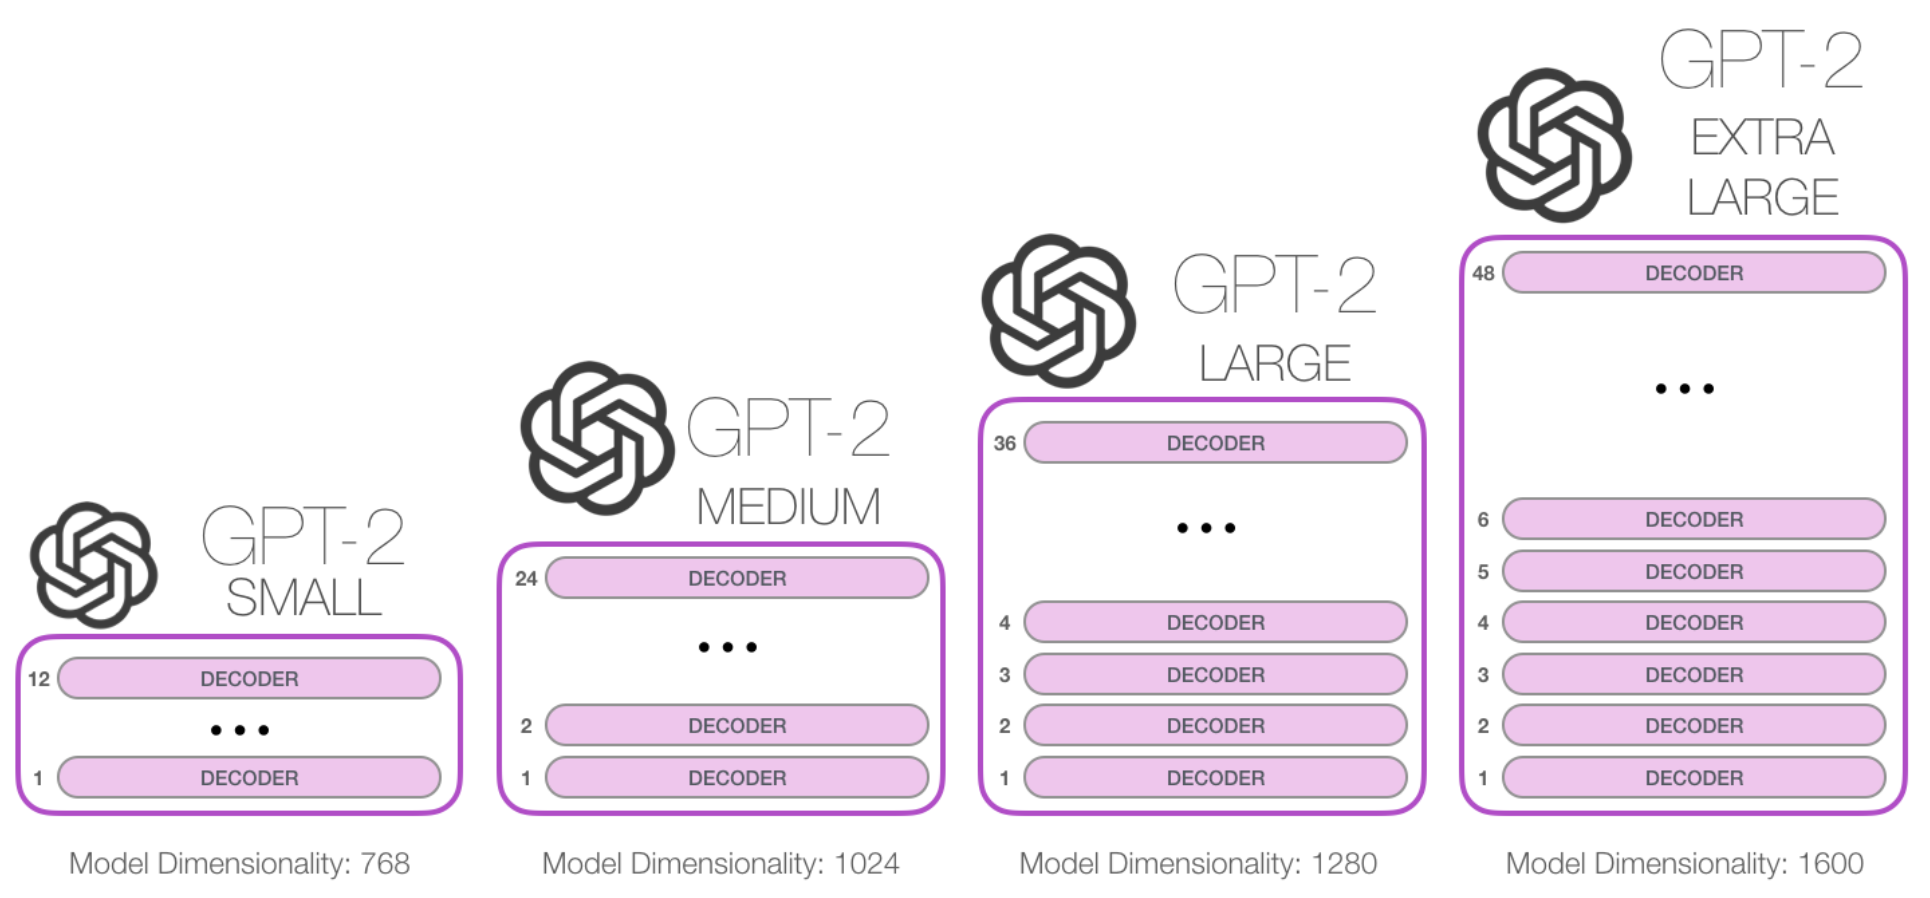
\includegraphics[width=0.85\textwidth]{figure/GPTModel}
    \caption{Possiamo vedere nell'immagine le varie tipologie di modelli di GPT-2, qui vi sono a seconda della grandezza diverse dimensioni del modello, utilizzando più decoder a seconda della grandezza del modello stesso.}
    \label{fig:GPTModel}
\end{figure}

\subsection{Architettura e funzionamento}

GPT è un modello Transformer unidirezionale, ovvero genera una parola alla volta considerando solo il contesto precedente. Il principio fondamentale è l'autoregressione: il modello predice la parola successiva $x_t$ data la sequenza delle parole precedenti $(x_1, x_2, ..., x_{t-1})$.

\subsubsection{Input e Tokenizzazione}

\begin{itemize}
    \item Il testo viene tokenizzato mediante una tecnica di tipo Byte-Pair Encoding (BPE);
    \item Ogni token viene convertito in un vettore di embedding;
    \item Viene aggiunto un \textit{positional embedding} per conservare l’informazione sull’ordine dei token;
    \item A differenza di BERT, non viene inserito alcun token [CLS] o [SEP], poiché GPT non è progettato per la classificazione o il confronto fra frasi.
\end{itemize}

\subsubsection{Decoder e Self-Attention causale}

GPT utilizza unicamente blocchi decoder del Transformer. Ogni blocco è composto da:
\begin{itemize}
    \item \textbf{Masked Self-Attention}: l'attenzione è limitata ai soli token precedenti mediante una \textit{causal mask}, impedendo al modello di vedere token futuri;
    \item \textbf{Feed-forward network} applicato a ciascun token individualmente;
    \item \textbf{Layer normalization} e \textbf{residual connections}, analogamente al Transformer standard.
\end{itemize}

\subsubsection{Output e Generazione}

\begin{itemize}
    \item Il vettore finale associato all’ultimo token viene proiettato nello spazio vocabolario tramite una matrice di output;
    \item Viene applicata una softmax per ottenere una distribuzione di probabilità sulle parole successive;
    \item Il token con la probabilità più alta può essere selezionato (greedy), oppure campionato (ad es. con temperature scaling o nucleus sampling);
    \item Questo processo viene iterato per generare una sequenza coerente parola dopo parola.
\end{itemize}

\subsection{Scelta del Token successivo}
Una volta che viene effettuato tutto il processo di analisi attraversando i decoder, ciò che viene generato alla fine è un vettore in cui sono presenti diverse probabilità di preddizione relative alla parola successiva della nostra frase, per scegliere di quale parola si tratta ci sono varie modalità adottate:

\begin{itemize}
    \item\textbf{Argmax}: Scelto il token con probabilità massima;
    \item\textbf{Sampling}: Si estra un token a caso, seguendo la distribuzione di probabilità fornita;
    \item\textbf{Top-k sampling}: Si considerano solo i top-k token probabili, per poi selezionare il token fra questi;
    \item\textbf{Top-p nucleus sampling}: Vengono considerati solo i token la cui somma delle probabilità supera un valore $p$, per poi selezionare un token fra questi in maniera casuale;
    \item\textbf{Beam Search}: Vengono mantenute più sequenze candidate contemporaneamente, il costo computazionale è elevato;
\end{itemize}

\begin{Osservazione}
    L'argmax, è una specializzazione del Top-k sampling, dove il valore di k è unitario.
\end{Osservazione}

\subsection{Pretraining}

GPT viene pre-addestrato in modo non supervisionato su un ampio corpus testuale, ottimizzando la funzione di perdita cross-entropy per predire il token successivo:
\[
\mathcal{L} = -\sum_{t=1}^{T} \log P(x_t \mid x_1, ..., x_{t-1})
\]
Non vi è masking di token né predizione bidirezionale: il modello impara a generare testo in modo fluente e coerente, acquisendo conoscenza grammaticale, lessicale e semantica implicita.

\subsection{Utilizzo in downstream tasks}

GPT può essere adattato a compiti specifici in due modalità:

\begin{itemize}
    \item \textbf{Fine-tuning supervisionato}: il modello viene addestrato su dataset etichettati per compiti come classificazione, QA, traduzione, ecc. (tipico in GPT-2);
    \item \textbf{Prompt-based learning}: grazie alla sua natura generativa, GPT può essere utilizzato in modalità \textit{zero-shot}, \textit{few-shot} o \textit{one-shot}, semplicemente modificando il prompt di input per adattarsi al task desiderato (approccio introdotto con GPT-3).
\end{itemize}

\begin{table}
    \centering
    \caption{Confronto tra BERT e GPT.}
    \begin{adjustbox}{width=\textwidth}
    \begin{tabular}{|l|c|c|}
    \hline
    \textbf{Caratteristica} & \textbf{BERT} & \textbf{GPT} \\
    \hline
    Architettura & Encoder Transformer & Decoder Transformer \\
    Direzionalità & Bidirezionale & Unidirezionale (autoregressivo) \\
    Obiettivo pretraining & MLM + NSP & Language Modeling \\
    Token speciali & [CLS], [SEP], [MASK] & Nessuno \\
    Uso principale & Comprensione del linguaggio & Generazione del linguaggio \\
    Modalità di utilizzo & Fine-tuning, feature extraction & Prompting, fine-tuning \\
    \hline
    \end{tabular}
    \end{adjustbox}
\end{table}
\section*{Approfondimenti}
\section{Varianti dei modelli Transformer}

Nel corso degli anni, numerose varianti dell’architettura Transformer sono state sviluppate per migliorarne l’efficienza, la generalizzazione e l’adattabilità a specifici compiti. Di seguito si riportano alcune delle più rilevanti:

\subsection{RoBERTa (Robustly Optimized BERT Approach)}

RoBERTa è una versione migliorata di BERT, introdotta da Facebook AI, che elimina l’obiettivo NSP, utilizza una maggiore quantità di dati e addestra il modello più a lungo. Le principali modifiche includono:
\begin{itemize}
    \item Rimozione del Next Sentence Prediction (NSP);
    \item Addestramento su batch più grandi e sequenze più lunghe;
    \item Dinamica del masking modificata ad ogni epoca.
\end{itemize}
RoBERTa ha mostrato prestazioni superiori a BERT in numerosi benchmark NLP.

\subsection{ALBERT (A Lite BERT)}

ALBERT propone un modello più leggero e scalabile mediante:
\begin{itemize}
    \item Condivisione dei pesi tra i layer;
    \item Fattorizzazione della matrice di embedding;
    \item Nuovo obiettivo di pretraining: \textit{Sentence Order Prediction (SOP)}.
\end{itemize}
Queste modifiche riducono drasticamente il numero di parametri, rendendo ALBERT più efficiente senza compromettere l’accuratezza.

\subsection{GPT-2, GPT-3 e GPT-4}

Le versioni successive della famiglia GPT hanno introdotto miglioramenti principalmente attraverso la scala del modello:
\begin{itemize}
    \item \textbf{GPT-2} (2019): 1.5 miliardi di parametri, addestrato su un ampio corpus web;
    \item \textbf{GPT-3} (2020): 175 miliardi di parametri, addestrato in modo da supportare \textit{few-shot} e \textit{zero-shot learning};
    \item \textbf{GPT-4} (2023): architettura multimodale, maggiore robustezza e comprensione contestuale, con performance avanzate su molteplici benchmark.
\end{itemize}

\subsection{ChatGPT e InstructGPT}

\begin{itemize}
    \item \textbf{InstructGPT} è una versione di GPT-3 fine-tunata mediante \textit{reinforcement learning from human feedback} (RLHF) per seguire istruzioni umane;
    \item \textbf{ChatGPT} è un'applicazione conversazionale basata su InstructGPT/GPT-3.5 o GPT-4, ottimizzata per generare risposte fluide, coerenti e utili in scenari di dialogo.
\end{itemize}

\subsection{Altri modelli noti}

\begin{itemize}
    \item \textbf{DistilBERT}: versione compressa di BERT, con il 40\% di parametri in meno e il 97\% delle performance;
    \item \textbf{ELECTRA}: introduce un pretraining discriminativo invece del classico MLM;
    \item \textbf{T5 (Text-to-Text Transfer Transformer)}: unifica i compiti NLP in un’unica formulazione testuale.
\end{itemize}

\section{Applicazioni pratiche dei Transformer}

L’adattabilità dei modelli Transformer consente la loro applicazione in una vasta gamma di task di NLP, sia in modalità supervisionata (fine-tuning) che non supervisionata (prompt engineering):

\begin{itemize}
    \item \textbf{Classificazione testuale}: assegnazione di etichette a frasi, documenti, tweet, ecc. (es. analisi del sentiment);
    \item \textbf{Named Entity Recognition (NER)}: identificazione di entità rilevanti nel testo (nomi, date, organizzazioni);
    \item \textbf{Risposta a domande (QA)}: estrazione o generazione di risposte date una domanda e un contesto;
    \item \textbf{Traduzione automatica}: conversione da una lingua a un’altra (es. inglese → francese);
    \item \textbf{Generazione di testo}: produzione di frasi o paragrafi coerenti a partire da un prompt (storytelling, copywriting);
    \item \textbf{Riassunto automatico}: estrazione o generazione di versioni sintetiche di testi lunghi;
    \item \textbf{Conversational AI}: chatbot e assistenti virtuali, spesso costruiti su InstructGPT o ChatGPT;
    \item \textbf{Codice e programmazione}: generazione di codice (es. Codex), spiegazione di funzioni o completamento automatico.
\end{itemize}

\section{Evoluzione dei Transformer}

L’evoluzione dei modelli Transformer è stata caratterizzata da un rapido progresso sia in termini di architettura che di scala computazionale. Di seguito è riportata una timeline dei principali modelli:

\begin{itemize}
    \item \textbf{2017 – Transformer} \cite{vaswani2017attention}: introduzione dell’architettura self attentiva in "Attention is All You Need".
    \item \textbf{2018 – BERT} \cite{devlin2018bert}: encoder bidirezionale pre-addestrato con obiettivi MLM e NSP.
    \item \textbf{2019 – GPT-2} \cite{radford2019language}: modello autoregressivo di grandi dimensioni per generazione testuale.
    \item \textbf{2019 – RoBERTa} \cite{liu2019roberta}: ottimizzazione di BERT tramite addestramento più esteso e rimozione NSP.
    \item \textbf{2019 – DistilBERT} \cite{sanh2019distilbert}: distillazione di BERT per maggiore efficienza.
    \item \textbf{2020 – T5} \cite{raffel2020exploring}: approccio "text-to-text" per unificare i compiti NLP.
    \item \textbf{2020 – GPT-3} \cite{brown2020language}: 175 miliardi di parametri, abilità few-shot learning.
    \item \textbf{2020 – ELECTRA} \cite{clark2020electra}: discriminatore al posto di un tradizionale generatore.
    \item \textbf{2021 – InstructGPT} \cite{ouyang2022training}: RLHF per migliorare l’allineamento con le intenzioni umane.
    \item \textbf{2022 – ChatGPT}: versione ottimizzata per il dialogo basata su InstructGPT.
    \item \textbf{2023 – GPT-4}: modello multimodale con prestazioni avanzate in molti contesti.
\end{itemize}



